% Standalone TikZ for fast iteration; final include via \input{} in jsac2_v1.tex
\documentclass[border=4pt,tikz]{standalone}
\usepackage{amsmath,amssymb}
\usepackage{bm}
\usepackage[T1]{fontenc}
\usepackage{lmodern}
\usepackage{tikz}
\usetikzlibrary{positioning,arrows.meta,calc,fit,backgrounds,shapes.geometric}

\definecolor{netblue}{HTML}{1F4E79}
\definecolor{twinorange}{HTML}{B26A00}
\definecolor{usergreen}{HTML}{2E7D32}

\begin{document}

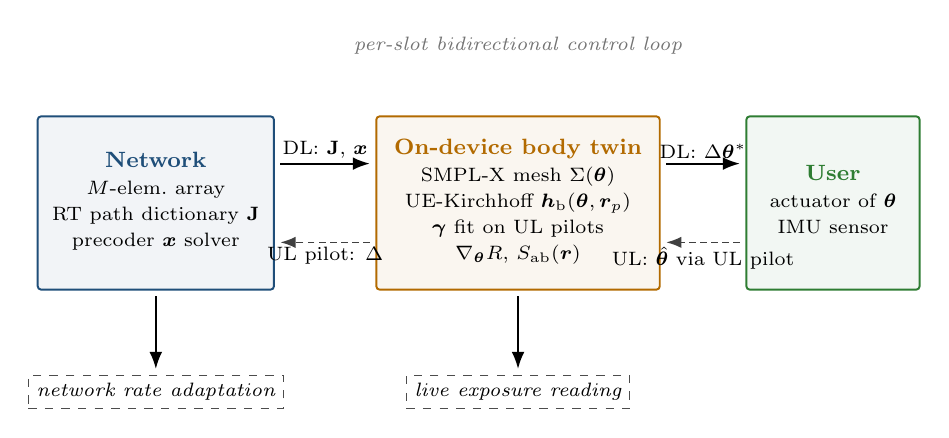
\begin{tikzpicture}[
    every node/.style={font=\footnotesize},
    bsbox/.style={draw=netblue, line width=0.7pt, rectangle, rounded corners=1.2pt,
                  inner sep=4pt, minimum height=22mm, minimum width=30mm,
                  fill=netblue!6, align=center},
    twin/.style={draw=twinorange, line width=0.7pt, rectangle, rounded corners=1.2pt,
                 inner sep=4pt, minimum height=22mm, minimum width=36mm,
                 fill=twinorange!6, align=center},
    user/.style={draw=usergreen, line width=0.7pt, rectangle, rounded corners=1.2pt,
                 inner sep=4pt, minimum height=22mm, minimum width=22mm,
                 fill=usergreen!6, align=center},
    output/.style={draw=black!70, line width=0.4pt, rectangle, dashed,
                   inner sep=3pt, fill=white, align=center, font=\scriptsize\itshape},
    farrow/.style={->, line width=0.7pt, >=Latex, shorten >=2pt, shorten <=2pt, color=black},
    barrow/.style={->, line width=0.55pt, >=Latex, shorten >=2pt, shorten <=2pt, color=black!75, dash pattern=on 2.5pt off 1.5pt},
    chlabel/.style={font=\scriptsize, align=center, inner sep=1.5pt,
                    text=black}
]

\node[bsbox] (bs) at (0, 0)  {\textbf{\color{netblue}Network}\\
    \scriptsize\strut $M$-elem.\ array\\
    \scriptsize\strut RT path dictionary $\mathbf{J}$\\
    \scriptsize\strut precoder $\bm{x}$ solver};

\node[twin]  (tw) at (4.6, 0) {\textbf{\color{twinorange}On-device body twin}\\
    \scriptsize\strut SMPL-X mesh $\Sigma(\bm{\theta})$\\
    \scriptsize\strut UE-Kirchhoff $\bm{h}_{\mathrm{b}}(\bm{\theta},\bm{r}_p)$\\
    \scriptsize\strut $\bm{\gamma}$ fit on UL pilots\\
    \scriptsize\strut $\nabla_{\bm{\theta}} R$, $S_{\mathrm{ab}}(\bm{r})$};

\node[user]  (us) at (8.6, 0) {\textbf{\color{usergreen}User}\\
    \scriptsize\strut actuator of $\bm{\theta}$\\
    \scriptsize\strut IMU sensor};

% --- Channel arrows: forward solid, return dashed ---
\draw[farrow] ([yshift=5mm]bs.east)  -- node[chlabel,above] {DL: $\mathbf{J}$, $\bm{x}$}
              ([yshift=5mm]tw.west);
\draw[barrow] ([yshift=-5mm]tw.west) -- node[chlabel,below] {UL pilot: $\Delta$}
              ([yshift=-5mm]bs.east);

\draw[farrow] ([yshift=5mm]tw.east)  -- node[chlabel,above] {DL: $\Delta\bm{\theta}^{*}$}
              ([yshift=5mm]us.west);
\draw[barrow] ([yshift=-5mm]us.west) -- node[chlabel,below] {UL: $\hat{\bm{\theta}}$ via UL pilot}
              ([yshift=-5mm]tw.east);

% --- Two semantic outputs ---
\node[output] (rate) at ($(bs)+(0,-2.4)$) {network rate adaptation};
\node[output] (read) at ($(tw)+(0,-2.4)$) {live exposure reading};

\draw[farrow] (bs.south) -- (rate.north);
\draw[farrow] (tw.south) -- (read.north);

% --- Loop direction annotation ---
\node[font=\scriptsize\itshape, color=black!55, align=center]
     at (4.6, 2.0) {per-slot bidirectional control loop};

\end{tikzpicture}

\end{document}
